\chapter{\ifenglish Introduction\else บทนำ\fi}

\section{\ifenglish Project rationale\else ที่มาของโครงงาน\fi}
ในปัจจุบัน, นักลงทุนมีการใช้การวิเคราะห์ทางเทคนิค (Technical Analysis) เพื่อช่วยให้การซื้อขายสินทรัพย์ในระยะสั้นได้กำไรสูงสุดเท่าที่เป็นไปได้
ซึ่งก็มักจะมีการใช้ตัวชี้วัดทางเทคนิค (Technical Indicators) หลายๆ อัน ในการที่จะพยายามหาจุดเข้าซื้อ หรือจุดขาย โดย 
ตัวชี้วัดทางเทคนิคเหล่านี้ส่วนใหญ่แล้วเป็นการคำนวณทางสถิติที่ใช้ ราคาย้อนหลัง, ปริมาณการซื้อขายย้อนหลัง, หรืออื่นๆ ในการ
คำนวณค่ามาเพื่อที่จะพยายามทำนายทิศทางของตลาด ซึ่งเราสามารถตีความหมายค่าของตัวชี้วัดทางเทคนิคด้วยเกณฐ์บางอย่าง เช่น 
สำหรับ RSI (Relative Strength Index) วิธีตีความหมายโดยทั่วไปคือ ถ้า RSI มากกว่า 70 หมายความว่าตลาดอยู่ใน
ภาวะซื้อมากเกินไปให้ขาย และถ้า RSI น้อยกว่า 30 หมายความว่าตลาดอยู่ในภาวะขายมากเกินไปให้เข้าซื้อ

ผู้จัดทำคิดว่าสามารถทำได้ดีกว่าการตีความหมายแบบในตัวอย่างก่อนหน้านี้ โดยใช้ Fuzzy Rule ในการตีความหมายจะให้ผลลัพธ์ที่ดีกว่าเนื่องจากตลาด
ซื้อขายสินทรัพย์น้้นมีความผันผวนและไม่แน่นอน ซึ่ง Fuzzy Logic นั้นสามารถทำงานได้ดีในการตีความ และใช้ข้อมูลที่คลุมเครือและไม่แน่นอน
นอกจากนี้ในงานวิจัยของ \cite{Rodrigo} ก็มีการใช้ Fuzzy Logic ในการระบบการซื้อขายสินทรัพย์ที่สำหรับจังหวะการเข้าซื้อ
และการจัดการเงินทุน ซึ่งทำงานได้ดีในตลาด NASDAQ100 และ EUROSTOXX ใน \cite{Escobar} ก็มีการใช้ Fuzzy Logic
ในการสร้างตัวชี้วัดทางเทคนิคจากการรับความเสี่ยงของผู้ใช้, ข้อมูลของตลาด, และอื่นๆ ซึ่งได้ผลลัพธ์ว่าตัวชี้วัดทางเทคนิคจาก Fuzzy Logic
มีประสิทธิภาพมากกว่าตัวชี้วัดทางเทคนิคแบบปกติ ได้แก่ MA, RSI และ MACD

ผู้จัดทำจึงได้สร้างระบบในการสร้างตัวชี้วัดทางเทคนิคใหม่จากตัวชี้วัดทางเทคนิค เช่น MACD, RSI, และอื่นๆ ด้วย Fuzzy Logic และสร้างระบบการจัดการเงินทุนด้วย
optimal-F ทีดัดแปลงให้ใช้ตัวชี้วัดทางเทคนิคที่มาจาก Fuzzy Logic (อ้างอิงจาก \cite{Rodrigo}) เพื่อช่วยในการตัดสินใจซื้อขายสินทรัพย์ให้ได้กำไรมากยิ่งขึ้น
โดยระบบทั้งหมดนี้จะมีเว็บแอปพลิเคชันที่จะรองรับการใช้งานทั้งในคอมพิวเตอร์และโทรศัพท์มือถือ เป็นอินเตอร์เฟซในการใช้งาน โดยผู้จัดจะทำตัวชี้วัดจาก Fuzzy Logic นี้บน 2 ตลาดก็คือตลาดหุ้น NASDAQ และตลาด Crypto-Currency
เพื่อเปรียบเทียบความแตกต่างของผลลัพธ์ในตลาดที่มีความผันผวนต่างกัน และมีความถึ่ของข้อมูลที่แตกต่างกัน

\section{\ifenglish Objectives\else วัตถุประสงค์ของโครงงาน\fi}
\begin{enumerate}
    \item เพื่อพัฒนา Fuzzy Logic ร่วมกับ Particle Swarm Optimization (PSO) สำหรับการสร้างวิธิการซื้อขายเฉพาะของแต่ละสินทรัพย์
    \item เพื่อสร้างเว็บแอปพลิเคชันเพื่อให้ผู้ใช้งานสามารถใช้งานระบบได้
\end{enumerate}

\section{\ifenglish Project scope\else ขอบเขตของโครงงาน\fi}
ข้อมูลที่ใช้งานคือข้อมูลของตลาดหุ้น NASDAQ ที่ได้มาจาก AlphaVantage (และ Finnhub) ในช่วงประมาณไตรมาสแรกของปี 2021 ถึงปัจจุบัน โดยมีของบริษัท TSLA, NKE, และ JPM 
และข้อมูลของตลาด Crypto-Currency จาก Binance โดยมี BTC, ETH และ BNB ในช่วงตั้งแต่ที่ Binance มีข้อมูลให้ 
รูปแบบของข้อมูลจะอยู่ในรูปของแท่งเทียนซึ่งมี ราคาเปิด, ราคาสูงสุด, ราคาต่ำสุด, ราคาปิด, และปริมาณการซื้อขาย ในช่วงเวลา 1 ชั่วโมง 

\section{\ifenglish Expected outcomes\else ประโยชน์ที่ได้รับ\fi}
เว็บแอปพลิเคชันที่สามารถโชว์ตัวชี้วัดทางเทคนิคจาก Fuzzy Logic ของเราทั้งที่ได้มาจากการปรับแต่งด้วย PSO และแบบที่จัดทำขึ้นมาเอง 
โดยมี UI ให้ user ปรับแต่ง Fuzzy Logic ต่างๆ เองได้ และมีราคาสินทรัพย์ที่อยู่ในรูปแบบแท่งเทียนโชว์อยู่ด้วย

\section{\ifenglish Technology and tools\else เทคโนโลยีและเครื่องมือที่ใช้\fi}
\begin{enumerate}
    \item Actix (Web Server Framework), Rust: สำหรับพัฒนาในส่วนของ Backend, การฝึกสอน Model, และ API ไว้ติดต่อกับ Frontend
    \item SvelteKit (Web Application Framework), Typescript: สำหรับพัฒนา Frontend ในส่วนของหน้าเว็บแอปพลิเคชัน
    \item MongoDB: สำหรับเก็บข้อมูลตลาดสินทรัพย์ที่เอาไว้ใช้ในการฝึกสอน Model, ใช้ในการแสดงบน Frontend และเก็บ Model ที่ฝึกสอนแล้ว
\end{enumerate}

%\section{\ifenglish Project plan\else แผนการดำเนินงาน\fi}

% \begin{plan}{1}{2023}{3}{2023}
%     \planitem{1}{2023}{1}{2023}{การทดลองโค้ดส่วนของ Backend}
%     \planitem{1}{2023}{1}{2023}{การทดลองโค้ดส่วนของ Frontend}
%     \planitem{2}{2023}{2}{2023}{ออกแบบ UI/UX}
%     \planitem{2}{2023}{3}{2023}{การพัฒนาระบบต้นแบบ}
%     \planitem{3}{2023}{3}{2023}{สรุปผลเป็นรูปเล่ม}
% \end{plan}

%\begin{figure}[ht]
    %\centering
    %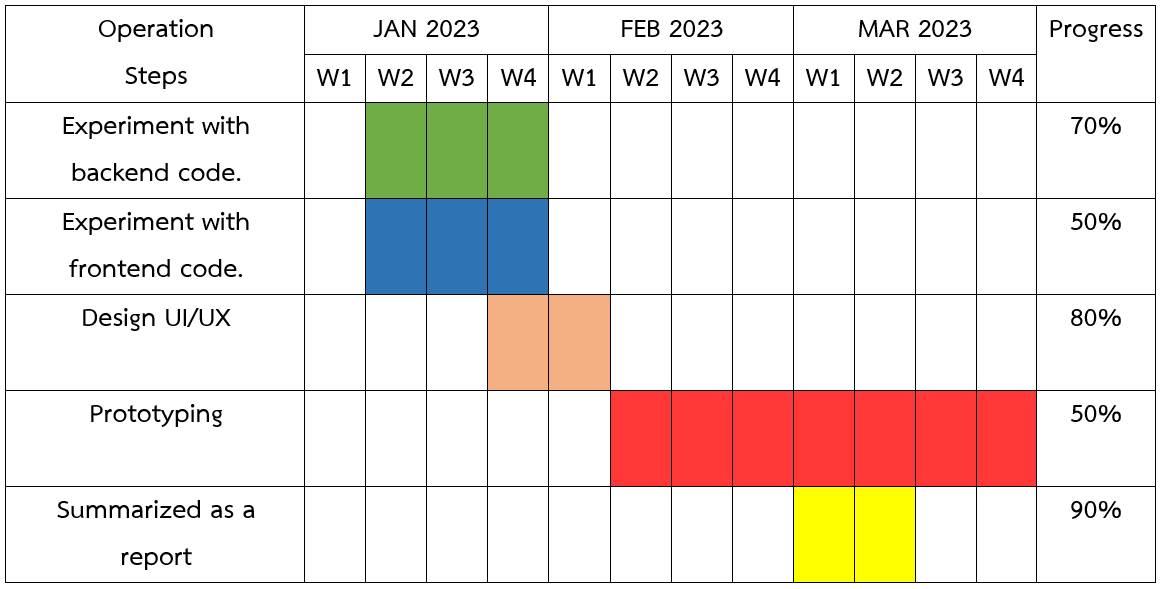
\includegraphics[width=\textwidth]{images/plan_progress.png}
%\end{figure}


\section{\ifenglish Roles and responsibilities\else บทบาทและความรับผิดชอบ\fi}
\begin{itemize}
    \item นายธนัตถ์ ตั้งอั้น รหัส 630610737 ทำในส่วนของ Backend โดยมีองค์ประกอบหลักๆ ก็คือตัวเว็บเซิฟเวอร์, database, การคำนวณ fuzzy logic และตัวชี้วัดทางเทคนิคต่างๆ และ
การปรับแต่ง fuzzy logic ด้วย PSO
    \item นายธนวัตน์ บำเพ็งพันธุ์ รหัส 630610736 ทำในส่วนของ Frontend คือการออกแบบ UI/UX, สร้างเว็บแอปพลิเคชันที่รองรับทั้งคอมพิวเตอร์และโทรศัพท์มือถือเพื่อติดต่อกับผู้ใช้งาน และบริการเว็บเซิฟเวอร์
\end{itemize}

\section{\ifenglish%
Impacts of this project on society, health, safety, legal, and cultural issues
\else%
ผลกระทบด้านสังคม สุขภาพ ความปลอดภัย กฎหมาย และวัฒนธรรม
\fi}
ระบบนี้อาจจะสามารถต่อเติมด้วยการใส่ตัวชี้วัดทางเทคนิคอื่นๆ ที่อาจจะมาจากแหล่งต่างๆมาเพื่มความละเอียดในการวิเคราะห์บางอย่าง
ซึ่งถ้าระบบนี้สำเร็จ ระบบนี้อาจจะเป็นเครื่องมือสำคัญให้กับนักลงทุนหลายๆคน และสามารถช่วยสร้างกำไรให้นักลงทุนเพิ่มได้ 